\begin{figure*}[t]
    \centering
    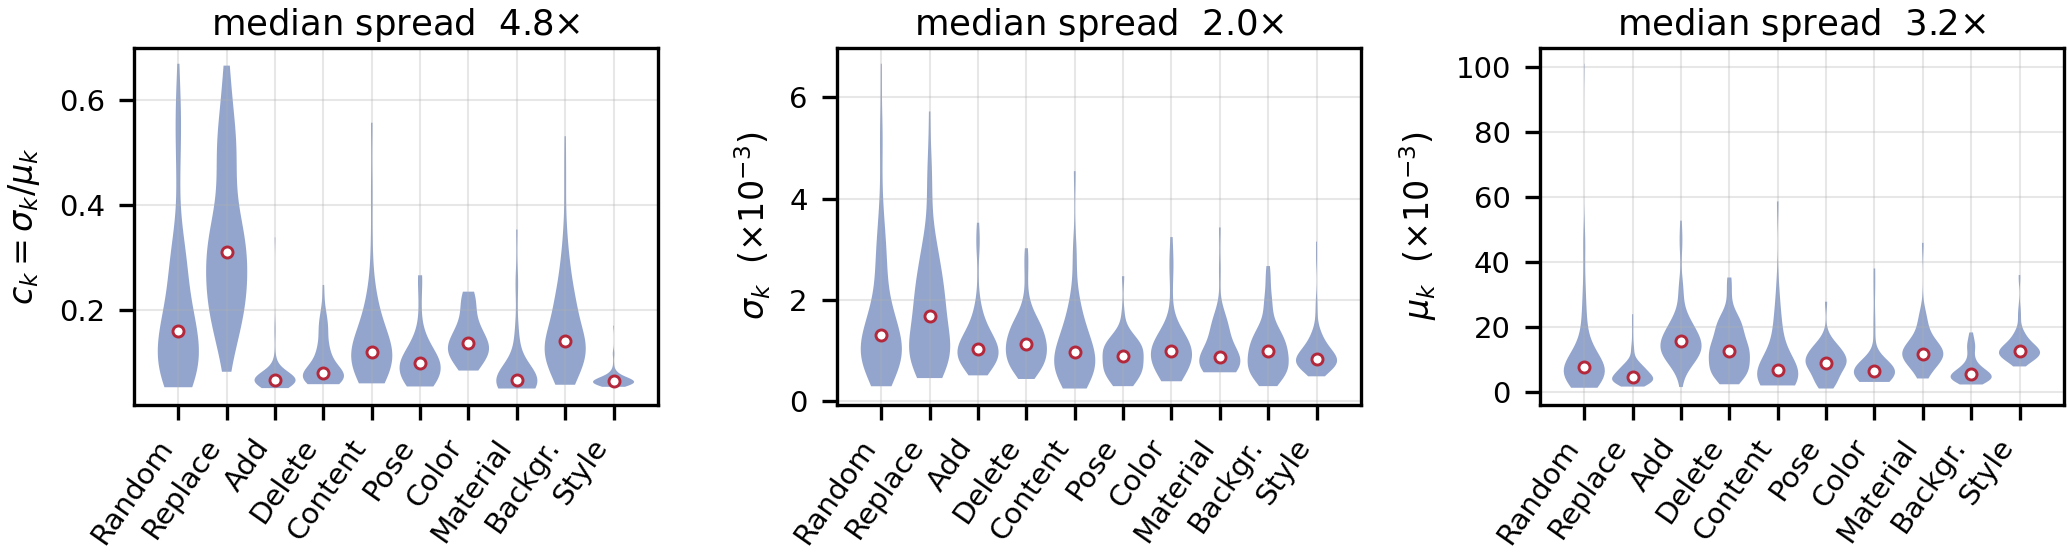
\includegraphics[width=\textwidth]{imgs/fig_cv_decomposition.png}
    \caption{What the coefficient of variation actually measures, over the 700 PIE-Bench cases at the last generation scale ($64{\times}64$). Violins show the per-category distribution; the marker is the median. \textbf{Left:} $c_k$ varies by a factor of $4.8$ between categories. \textbf{Middle:} its numerator $\sigma_k$ varies by only $2.0$. \textbf{Right:} its denominator $\mu_k$ varies by $3.2$, in the direction \emph{opposite} to $c_k$ --- the categories with the lowest $c_k$ (object addition, style transfer) are exactly those with the highest $\mu_k$. The between-category signal in $c_k$ is therefore carried almost entirely by the mean, i.e.\ by how large a fraction of the image the focus region occupies, and not by the shape of the distribution.}
    \label{fig:cv_decomposition}
\end{figure*}
